\chapter{SYSTEM DESIGN}

This document specifies the detailed design of the “Mystery Doors” project.  It deals  with  system  overview  of  the  overall  project,  proposed  architecture  designs  and alternate  architecture  design  and  justification  for  the  proposed  one.  High  level  block diagrams which  illustrates  the  database  and  application  program  interaction. High level use case report which includes all users and interaction between them. Low level design of each module consists individual use case reports, and related sub-module sequence diagrams, activity diagrams, pseudo code, Analysis and Asymptotic Notation for algorithms.

\section{System Overview}
\hspace{1cm}GUI contains the welcome screen or main menu screen which must consist of two buttons. PLAY and EXIT. If user clicks on EXIT button the game must terminate. When user clicks on PLAY button, he/she must be given an option to enable or disable sound. If user enables sound then background audio need to be played using background audio player agent. 
When user clicks on PLAY button the game must navigate to next page showing the introduction to game using motion of characters. Characters are moved using motion of images(.gif to enable animation). During gameplay different set and type of questions need to displayed on screen and answers must be validated before proceeding to next step. Different set and type of questions and all the solutions must be stored in an isolated file storage medium i.e. mobile’s flash memory. At a different level’s of game suitable type of question must be fetched from file and displayed on screen.


\section{Design Aspects}
\hspace{1cm}
                            The goal of this design is to ensure that the architecture is preserved, and the relationship between the component and modules is clear.  This design views the modules as classes. Object oriented approaches are believed to be more natural and provide richer structures for thinking and abstraction. As we are using C sharp  programming language which is truly object oriented languages.

\subsection{Object Oriented Design}
\hspace{1cm}During object-oriented design (OOD), a developer applies
implementation constraints to the conceptual model produced in
object-oriented analysis. Such constraints could include not only
constraints imposed by the chosen architecture but also any
non-functional – technological or environmental – constraints, such as
transaction throughput, response time, run-time platform, development
environment, or those inherent in the programming language. Concepts
in the analysis model are mapped onto implementation classes and
interfaces resulting in a model of the solution domain, i.e., a
detailed description of how the system is to be built.
%==============================
\subsubsection{Activity Diagram}
\hspace{1cm} The fig.3.1 shows the activity diagram .It describes different activities performed by different components .
%You can add figure using the following syntax
\vspace {0.5cm}
\begin{figure}[htbp]
	\centering
	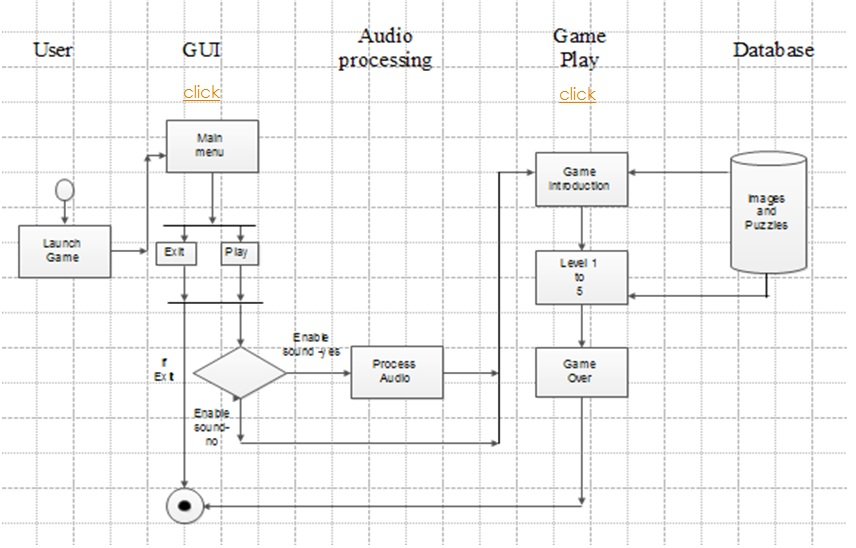
\includegraphics[width=10cm,height=8cm]{activity.jpg}
	\caption{Activity-diagram}
\end{figure}
\vspace{5cm}
%==============================
\subsubsection{Class Diagram}
\hspace{1cm}In fig.3.2 shows the Class diagram. Class diagram is a type of static structure diagram that describes the structure of a system by showing the system‟s classes, their attributes and the relationship between the classes. 
%You can add figure using the following syntax
\vspace {0.5cm}
\begin{figure}[htbp]
	\centering
	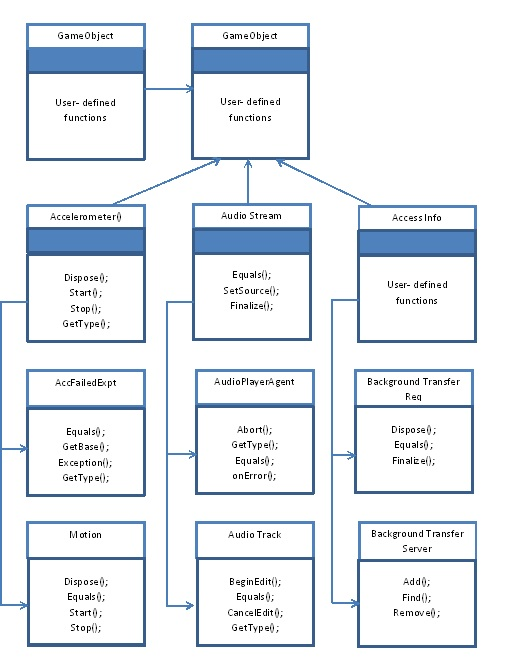
\includegraphics[width=10cm,height=6cm]{class.JPG}
	\caption{Class Diagram}\end{figure}
\paragraph\ \hspace{0.5cm} 
\vspace{5cm}
%==============================
\subsubsection{Sequence Diagram}
\hspace{1cm}The fig.3.3 shows how processes operate with one another and in what order 
with the help of sequence diagram
 
%You can add figure using the following syntax
\vspace {0.5cm}
\begin{figure}[htbp]
	\centering
	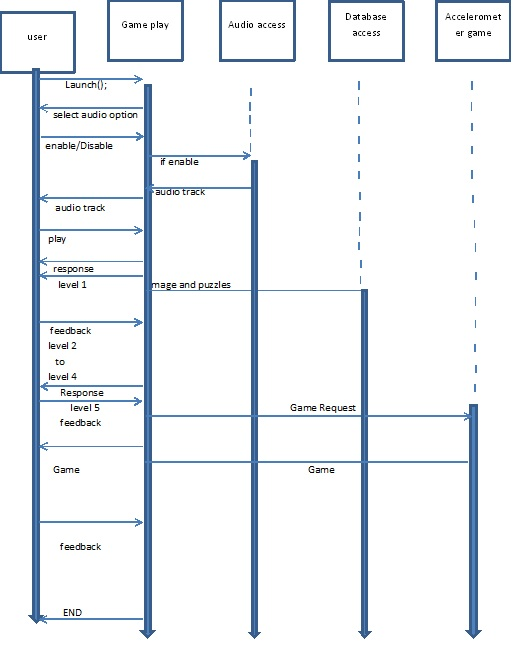
\includegraphics[width=10cm,height=6cm]{seq.jpg}
	\caption{Sequence Diagram}
\end{figure}
\paragraph\ 

%==============================================================

\section{Prototype Level Design}
\hspace{1cm}Since we have followed evolutionary prototyping method in developing our app, the system development happens in increments.Each prototype level design describes the incremental process followed in that phase of development.\\


%==============================
\subsection{Prototype : 1}
\hspace{1cm}When the player (Alex) gets to the first door, he encounters Dhaka. This level is used to make the player get acquainted to the game.  He should answer 3 different types of questions to open the 1st Mystery Door.
This section contains the 1st phase of the app development. Features implemented during this phase were:
\begin{itemize}
\item \textbf {}Gameplay till level 2.
\item \textbf {}Questions were based on General Knowledge, Visual question and tricky riddle
\item \textbf {}Editing of images for the characters in the story line
\end{itemize}
%==============================
\subsubsection{Algorithm for Gameplay}

\hspace{1cm}
This is the algorithm for Gameplay\\
\rmfamily\ 
ALGORITHM:GAME PLAY \\
//INPUT the buttons clicked (PLAY, EXIT)\\
//OUTPUT proper navigation of xaml pages corresponding to those buttons\\
Begin\\
If(button is assigned to the right xaml page)\\
Introductory page is displayed;\\
else\\
error;\\
End
\rmfamily

\subsubsection{Algorithm for introductory page}

 \hspace{1cm}This is the algorithm for Introductory page\\
\rmfamily\ ALGORITHM: intro page()\\
//INPUT the START button\\
//OUTPUT the motion of the images begin to give an introduction to the game\\
Begin\\
If(button-clicked)\\
Start the motion of the image and start the introduction;\\
else\\
no motion of the images;\\
end
\rmfamily
%==============================
\subsubsection{Algorithm for game levels }
 \hspace{1cm}This is the algorithm for Game levels
\rmfamily\ ALGORITHM: level one two()\\
//INPUT the correct answers and the CONTINUE button\\
//OUTPUT go to the next level\\
Begin\\
If(CONTINUE is clicked)\\
Go to the first level of the game;\\
Display the number of attempts;\\
Display the questions;\\
If(answers are right)\\
Notify the user;\\
Go to the next question or level;\\
Else\\
Notify the user about the wrong answer;\\
Decrement an attempt;\\
Else\\
Restart the game from the first level;\\
end
\rmfamily

%==============================

\subsection{Prototype : 2}
\hspace{1cm}When the player reaches the 3rd door, the level of difficulty increases. The player is provided a time constraint and the use of password. The player is provided with a different set of questions, through which he can unveil the password, the password revealed will be used to unlock the 3rd door.\\
This section contains the 2nd phase of the app development. Features implemented during this phase were:\\
Creation of level 3, 4 and 5
\begin{itemize}
\item \textbf {}Introducing the time-constraint in 3rd, 4th and 5th level.
\item \textbf {}Introducing the concept of “password”.
\end{itemize}
%==============================
\subsubsection{Algorithms for creation of level 3, 4 and 5 }
\hspace{1cm}Algorithm for Game Levels\\ 
\rmfamily\ 
ALGORITHM: rest levels ()\\
//INPUT the correct answers and the CONTINUE button\\
//OUTPUT continued to the next level and at the end a message to display\\
Begin\\
If(CONTINUE is clicked)\\
Go to the third level of the game;\\
Display the number of attempts;\\
Display the questions;\\
If(answers are right)\\
Notify the user;\\
Go to the next question or level;\\
Else\\
Notify the user about the wrong answer;\\
Decrement an attempt;\\
Else\\
Restart the game from the 3rd level;\\
end
\rmfamily

%==============================
\subsubsection{Algorithm for time-constraint }
 \hspace{1cm}
\rmfamily\ ALGORITHM: time ()\\
//INPUT  state where the user has completed 2 levels\\
//OUTPUT timer starts\\

Begin\\
 if (level==3 or 4 or 5)\\
start timer;\\
if(timer==120 or 100 or 75 seconds)\\
terminate level and goto level 3 ;\\
End
\rmfamily
%==============================
\subsubsection{Algorithm for  password generation }
\hspace{1cm}This algorithm is for password generation\\
\rmfamily\ 
ALGORITHM: password ()\\
//INPUT three correct answers\\
//OUTPUT 2 letters of the password are revealed after answering one question\\
Begin\\
For ( ques=3 ques<4 ques++)\\
Reveal 2 letters;\\
end
\rmfamily


%==============================

\subsection{Prototype : 3}
\hspace{1cm}This section contains the 3rd phase of the app development. Features implemented during this phase were:\\
\begin{itemize}
\item \textbf {}Introducing the concept of “life” in 3rd, 4th and 5th level.
\item \textbf {}Concept of “game over”.
\end{itemize}


%==============================
\subsubsection{Algorithm for bonus life option}
 \hspace{1cm}This algorithm is for bonus life option\\ 
\rmfamily\ ALGORITHM: life ()\\
//INPUT when the user completes a level\\
//OUTPUT Increase in life i.e.  displays a heart symbol at the top of the screen.\\
Begin\\
If (correct answer and 3 or 4 level is crossed)\\
Increment In life;\\
Else If (user loses 3 attempts)\\
Decrement a life;\\
Else \\
end
\rmfamily

\subsubsection{Algorithm for  game over}
\hspace{1cm}This algorithm is for game over\\
\rmfamily\ ALGORITHM: game over ()\\
//INPUT incorrect answers\\
//OUTPUT game over page\\
Begin\\
If (time exceeds the constraint or the lives are lost)\\
Display game over;\\
Display the button to RESTART and EXIT ;\\
Else\\
Continue the game;\\
Navigate the control to the last page;\\
end
\rmfamily
